% Shared body of submission.tex and arxiv.tex.
% Rules for this draft:
%  - every number comes from a generated file (benchmarks/paper/figures/*.tex, analysis CSVs,
%    committed JSONs); never retype one;
%  - main body <= 12 pages before references (longer = 4-week reviews);
%  - claims are scoped to what was run: homophilous citation graphs, one untuned shared
%    protocol, 10 seeds, the public split unless stated;
%  - no \todo may remain in either PDF (`make check`).

\begin{abstract}
\todo{One paragraph, written by you. It must state: the question (method vs.\ backbone vs.\
evaluation); the setup (7 objectives, GCN and GIN, Cora/CiteSeer/PubMed + ogbn-arxiv, 10 seeds,
untrained encoder of the same backbone as anchor); the three findings with one number each
(spread 4.9 vs 18.8 points on Cora; probe changes the gain several-fold, not the ranking;
implementation details move results as much as the objective); the headline variance share;
and the release of code and results.}
\footnote{\todo{Required by TMLR: a first-page footnote disclosing how large language models
were used (e.g.\ for code, literature search, editing). Write it precisely.}}
\end{abstract}

\section{Introduction}
\label{sec:intro}
\todo{Open with the problem: published graph-SSL comparisons mix encoders, budgets and probe
protocols (Table~\ref{tab:audit}), and rarely report the untrained encoder. Then the question,
then Figure~\ref{fig:headline}, then the contributions:
(1) a controlled study crossing method $\times$ backbone $\times$ probe $\times$ split with an
untrained anchor per backbone;
(2) an audit of the probe protocols of eight reference codebases;
(3) a variance decomposition that puts a number on ``how much is the method'';
(4) a reporting checklist, code and every result file.}

\begin{figure}[t]
  \centering
  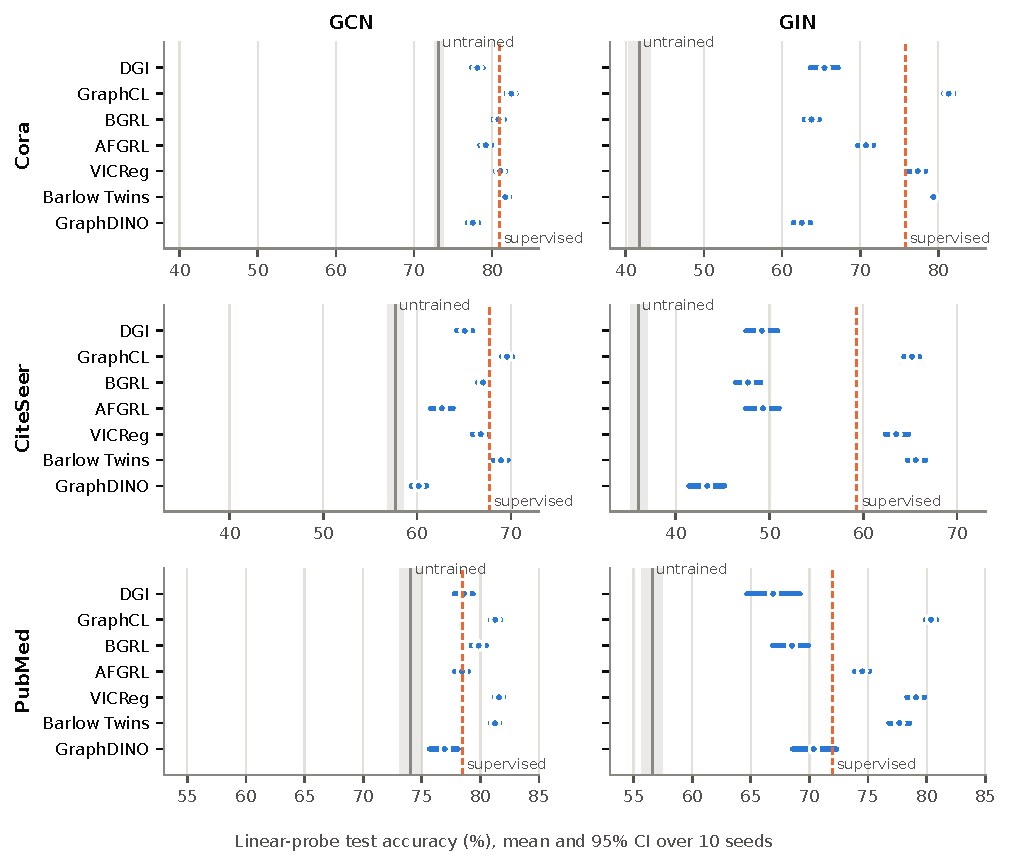
\includegraphics[width=\linewidth]{fig1_backbone_vs_method}
  \caption{\todo{Caption: what is plotted (mean and 95\% bootstrap CI over 10 seeds), the band
  (untrained encoder of the same backbone), the dashed line (supervised, standard recipe), and
  the one-sentence takeaway.}}
  \label{fig:headline}
\end{figure}

\section{Related work}
\label{sec:related}
\todo{Three paragraphs, each ending with how this paper differs.
(a) Evaluation critiques in graph learning, all supervised or non-SSL:
\citet{shchur2018pitfalls,errica2020fair,platonov2023heterophily,tonshoff2023gap,luo2024classic}.
(b) Graph-SSL evaluation, each fixing a factor we vary:
\citet{zhu2021pygcl} (encoder fixed), \citet{ma2024gcleval} (no backbone/probe axis, no untrained
anchor), \citet{xu2024graphfm}, \citet{song2025gstbench} (transfer setting),
\citet{trivedi2022augmentations,khanna2025untrained} (untrained baselines, graph level),
\citet{guo2023architecture,jian2024spectral,sun2022pretraining,wang2022molgrapheval}.
(c) SSL evaluation and variance outside graphs:
\citet{kolesnikov2019revisiting,goyal2019scaling,kornblith2019transfer,marks2024probing,dubois2023risk,bouthillier2021variance,hagmann2023reliability,agarwal2021precipice}.}

\section{Experimental setup}
\label{sec:setup}
\todo{Methods (\citet{velickovic2019dgi,you2020graphcl,thakoor2022bgrl,lee2022afgrl,bardes2022vicreg,zbontar2021barlow,caron2021dino});
encoders \citep{kipf2017gcn,xu2019gin}; the shared protocol (2 layers, 256 units, batch norm,
300 full-batch steps, AdamW $5\times10^{-4}$, edge drop 0.5 + feature mask 0.2); untrained
encoder = same architecture at initialisation; probes (Section~\ref{sec:probe}); public split
and 10 random 10/10/80 splits; 10 seeds; selection on validation only; hardware and commits.
State that GraphDINO uses reference DINO values and why.}

\section{The backbone sets the spread, not the leaders}
\label{sec:backbone}
\todo{Claim C1. Evidence: Table~\ref{tab:main}, Figure~\ref{fig:headline}, Kendall $\tau$
between GCN and GIN rankings (benchmarks/paper/analysis/kendall\_tau.csv), effective rank of
BGRL with each backbone.}

\begin{table}[t]
  \centering
  \small
  \caption{\todo{Caption: linear-probe test accuracy (mean $\pm$ std over 10 seeds) and gain
  $\Delta$ over the untrained encoder of the same backbone.}}
  \label{tab:main}
  % Generated by benchmarks/paper_figures.py from run_benchmark.py JSONs. Do not edit.
\begin{tabular}{llrrrrrr}
\toprule
Backbone & Method & \multicolumn{2}{c}{Cora} & \multicolumn{2}{c}{CiteSeer} & \multicolumn{2}{c}{PubMed} \\
 &  & Acc. & $\Delta$ & Acc. & $\Delta$ & Acc. & $\Delta$ \\
\midrule
GCN & \textit{Untrained} & 73.2 $\pm$ 1.0 &  & 57.7 $\pm$ 1.5 &  & 74.1 $\pm$ 1.6 &  \\
GCN & DGI & 78.1 $\pm$ 1.2 & +5.0 & 65.1 $\pm$ 1.4 & +7.4 & 78.6 $\pm$ 1.3 & +4.5 \\
GCN & GraphCL & 82.5 $\pm$ 1.1 & +9.3 & 69.6 $\pm$ 1.0 & +11.9 & 81.3 $\pm$ 0.8 & +7.2 \\
GCN & BGRL & 80.8 $\pm$ 1.2 & +7.6 & 67.1 $\pm$ 0.9 & +9.4 & 79.9 $\pm$ 1.1 & +5.8 \\
GCN & AFGRL & 79.2 $\pm$ 1.3 & +6.0 & 62.6 $\pm$ 2.0 & +4.9 & 78.4 $\pm$ 1.0 & +4.4 \\
GCN & VICReg & 81.1 $\pm$ 1.1 & +7.9 & 66.8 $\pm$ 1.4 & +9.1 & 81.6 $\pm$ 0.7 & +7.5 \\
GCN & Barlow Twins & 81.6 $\pm$ 0.9 & +8.5 & 69.0 $\pm$ 1.3 & +11.3 & 81.2 $\pm$ 0.7 & +7.2 \\
GCN & GraphDINO & 77.5 $\pm$ 1.2 & +4.4 & 60.2 $\pm$ 1.4 & +2.5 & 77.0 $\pm$ 2.1 & +2.9 \\
GCN & \textit{Supervised (std. recipe)} & 80.9 $\pm$ 0.8 & +7.7 & 67.7 $\pm$ 1.7 & +10.0 & 78.5 $\pm$ 0.9 & +4.4 \\
\midrule
GIN & \textit{Untrained} & 41.7 $\pm$ 2.4 &  & 36.1 $\pm$ 1.6 &  & 56.6 $\pm$ 1.5 &  \\
GIN & DGI & 65.4 $\pm$ 3.0 & +23.7 & 49.2 $\pm$ 2.9 & +13.1 & 66.9 $\pm$ 3.9 & +10.3 \\
GIN & GraphCL & 81.3 $\pm$ 1.1 & +39.6 & 65.2 $\pm$ 1.4 & +29.1 & 80.4 $\pm$ 0.8 & +23.8 \\
GIN & BGRL & 63.8 $\pm$ 1.6 & +22.1 & 47.7 $\pm$ 2.3 & +11.6 & 68.5 $\pm$ 2.6 & +11.9 \\
GIN & AFGRL & 70.7 $\pm$ 1.7 & +29.0 & 49.3 $\pm$ 3.0 & +13.3 & 74.5 $\pm$ 1.1 & +17.9 \\
GIN & VICReg & 77.4 $\pm$ 1.9 & +35.7 & 63.5 $\pm$ 2.1 & +27.5 & 79.1 $\pm$ 1.3 & +22.5 \\
GIN & Barlow Twins & 79.3 $\pm$ 0.8 & +37.6 & 65.6 $\pm$ 1.6 & +29.5 & 77.7 $\pm$ 1.5 & +21.1 \\
GIN & GraphDINO & 62.5 $\pm$ 1.9 & +20.8 & 43.3 $\pm$ 3.3 & +7.3 & 70.4 $\pm$ 3.2 & +13.8 \\
GIN & \textit{Supervised (std. recipe)} & 75.8 $\pm$ 2.3 & +34.1 & 59.3 $\pm$ 4.5 & +23.3 & 72.0 $\pm$ 1.9 & +15.4 \\
\bottomrule
\end{tabular}

\end{table}

\section{Every gain needs its own untrained anchor}
\label{sec:anchor}
\todo{Claim C2. The 31-point gap between untrained GCN and GIN; methods ending below the
anchor (BGRL with a batch-norm predictor on ogbn-arxiv; GraphDINO with reference values at
3,000 steps); untrained GCN-3L on ogbn-arxiv above every trained GIN-2L.}

\section{The probe changes the size of the gain, not the order}
\label{sec:probe}
\todo{Claim C3. Figure~\ref{fig:probes} (Planetoid, both backbones) and the ogbn-arxiv
comparison; Kendall $\tau$ of each probe against the converged one.}

\begin{table}[t]
  \centering
  \small
  \caption{Linear-evaluation protocols in reference implementations of graph SSL, read from
  their code on 2026-10-24 (default branch, commit in brackets).
  \todo{Re-check each row against the code before submission.}}
  \label{tab:audit}
  \begin{tabularx}{\linewidth}{l l X l}
    \toprule
    Codebase & Classifier and budget & Features and regularisation & Model selection \\
    \midrule
    DGI (\texttt{61baf67}) & Adam lr 0.01, 100 steps, 50 runs & raw; no weight decay & last step \\
    PyG-SSL (\texttt{7ab0f64}) & Adam lr 0.01, 100 steps, 50 runs & raw; no weight decay & last step; without masks val = test \\
    DIG sslgraph (\texttt{21476b0}) & Adam lr 0.01, 300 steps & raw; no weight decay & pre-training epoch by \textbf{test} accuracy \\
    GraphMAE (\texttt{b14f080}) & Adam lr 0.01, 300--600 steps & raw; weight decay per dataset & best validation \\
    PyGCL (\texttt{aa238b3}) & Adam lr 0.01, 5{,}000 steps & raw; no weight decay & best validation (every 20) \\
    GCA (\texttt{0f17497}) & Adam lr 0.01, 5{,}000 steps & raw; no weight decay & best validation; without val, best \textbf{test} \\
    GRACE (\texttt{b3b5ac3}) & liblinear, one-vs-rest & L2-normalised; $C$ by 5-fold CV on train & CV on train \\
    BGRL (\texttt{60f9f19}) & liblinear, one-vs-rest & L2-normalised; $C \in 2^{-10..10}$ & validation (preset splits) \\
    \midrule
    GraphSSL (ours) & L-BFGS to convergence & standardised; L2 grid $10^{-6..1}$ & validation \\
    \bottomrule
  \end{tabularx}
\end{table}

% \begin{figure}[t]
%   \centering
%   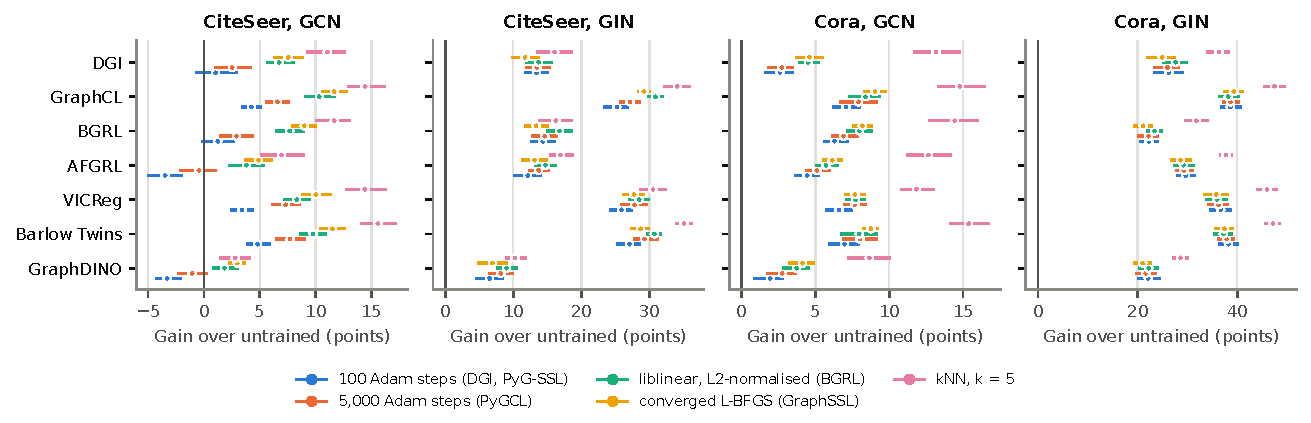
\includegraphics[width=\linewidth]{fig2_probe_protocols}
%   \caption{\todo{}}
%   \label{fig:probes}
% \end{figure}
% Uncomment once `bash benchmarks/paper_runs.sh probe` and `analyze` have run.

\section{Implementation details move results as much as the objective}
\label{sec:details}
\todo{Claim C4, one compact table with matched controls: predictor normalization (ogbn-arxiv,
3 seeds), GCN BatchNorm momentum, DGI one vs two passes, GraphDINO teacher values (selected on
test: say so), training budget 300 $\to$ 3{,}000 steps; same-seed reruns on two machines
(benchmarks/paper/analysis/reruns.csv). Each row: mechanism, or ``cause not identified''.
Precedents: \citet{engstrom2020implementation,henderson2018rl,richemond2020byolbn,he2020moco,wu2021batchnorm}.}

\section{How much is the method? A variance decomposition}
\label{sec:variance}
\todo{Share of variance explained by method, backbone, probe, split and interactions, on
accuracy and on gain over untrained (benchmarks/paper/analysis/variance\_shares.csv), with the
caveat that eta squared on a balanced design is descriptive.}

\section{Recommendations}
\label{sec:recommendations}
\todo{A short checklist, in your words. Candidates from the evidence: report the untrained
encoder of the same backbone; state the probe solver and whether it converged; use at least two
backbones or justify one; at least 10 seeds with intervals; select on validation only; report
effective rank as a diagnostic, not a target; state the training budget.}

\section{Limitations}
\label{sec:limitations}
\todo{Homophilous citation graphs (+ ogbn-arxiv); one untuned protocol; GraphDINO values chosen
on test; generative methods (GraphMAE) not covered; one seed per mini-batch model on ogbn-arxiv;
nondeterminism not decomposed by operation.}

\section{Conclusion}
\todo{Three or four sentences.}

\paragraph{Code and data.} Code, configurations and every per-seed result file are available
at \codeurl.

\bibliography{references}
\bibliographystyle{tmlr}

\appendix
\section{Per-seed results and provenance}
\todo{Rendered from the JSON files: commit, hardware and versions per row.}

\section{BGRL on ogbn-arxiv with the protocol of its paper}
\todo{The reproduction (71.32 vs 71.64 test) and the factor-difference table.}

\section{ZINC: frozen encoders and the number of seeds}
\todo{Half a page: frozen SSL $\approx$ untrained; 3 vs 10 seeds changed the conclusions. No
claim that pre-training helps after fine-tuning.}
